\chapter{Conceitos Básicos} %consertar organização do texto
Nesta seção, será explorado alguns fundamentos básicos para compreender, passo a passo, como será conduzida a metodologia proposta. Primeiramente introduz-se o problema da classificação de dados. Logo após esse conceito, descreve-se brevemente sobre uma abstração matemática muito utilizada na computação, o Grafo, que têm como serventia facilitar a visualização de como é composta a estrutura de um neurônio artificial, apresentada esta junto ao K-vizinhos mais próximos, como exemplos de técnicas de categorização de dados. Por fim, é apresentado uma introdução ao Processamento de Linguagem Natural (PLN), dando enfase um sub-conceito muito valioso para os objetivos deste trabalho, que é classificação de texto.

\section{Classificação de dados}
Classificação de dados é um problema que abrange enumeras aplicações em diversos tipos de cenários no nosso dia a dia, tais como diagnóstico de doenças, identificação de objetos em fotos e vídeos, categorização de seres vivos e espécies, dentre outros. Esse problema é um dos tópicos mais ativos na área de aprendizado de máquina. Isso se dá, porque classificar dados consiste em determinar um rótulo ou classe para um objeto, baseado em um conjunto de características extraídas do mesmo \citep{duda1973pattern,bishop2006pattern}. 

Em geral, dados são classificados como pertencentes a uma única classe ou categoria. Essa forma de classificação é denominada classificação de rótulo único. Por outro lado, se houver mais uma forma de rotular a mesma entrada, então dá-se o nome de classificação de multi-rótulo. 

Formalmente o processo de classificação consiste em $X = \{X_1,...,X_i\}$ um conjunto de $i$ entradas, $C = \{c_1,...,c_n\}$ um conjunto de $n$ classes, tal que $n \geq 2$, e $Y = \{(X_1, \{c_1,...,c_j\}),...,(X_i, \{c_n,...,c_k\})\}$ um conjunto de treinamento, no qual cada entrada $X_i$ é categorizada por uma ou mais classes $c_i$. O objetivo geral de um classificador é aprender, através de seu conjunto de treinamento $Y$, uma possível correlação entre os atributos das entradas com suas classes, de tal forma que para uma entrada $X' = \{X'_1,...,X'_i\}$ que não possua rótulo $c$ qualquer, seja possível classificar-lá.

Para ilustrar o processo de classificação de dados, considere o problema da flor de Iris. Nesse problema, existe um conjunto de flores do gênero Iris que podem ser rotuladas de uma das três maneiras: do tipo setosa, virgínica ou versicolor. Partindo desse ponto, o objetivo é determinar a qual grupo uma determinada flor pertence baseado nas medidas de sépalas e pétalas da mesma. A Figura \ref{fig:irisExample} ilustra o processo de classificação. Inicialmente as informações especificas sobre as sépalas e pétalas devem ser extraídas em um pré-processamento. Em seguida tais medidas são processadas e suas características extraídas. Por fim, é realizada a classificação das flores. Neste exemplo os valores de $X$ serão as medidas de comprimento, largura das sépalas e pétalas e $C$ assumirá os rótulos setosa, virgínica e versicolor.

Em geral, existem diversos algoritmos para classificação de dados, onde cada um possui sua especificidade, vantagens e desvantagens. Neste trabalho, aborda-se o uso de duas técnicas para classificação de dados, sendo elas RNA e KNN.

\begin{figure}[ht!]
\caption{Processo de classificação de flores do gênero Iris}
\label{fig:irisExample}
\centering
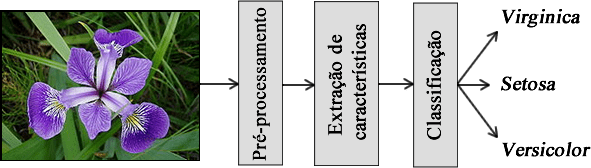
\includegraphics[scale=0.5]{img/irisExample.png}
{\fontsize{11pt}{\baselineskip}\selectfont
\\Fonte: \cite{pacheco2016agregaccao}
}
\end{figure}

\subsection{Grafos}
Muitas situações no mundo real podem ser descritas com o uso de um diagrama, composto por um conjunto de pontos e arestas, onde as arestas unem pares desses pontos. Por exemplo, os pontos podem representar cidades em um mapa, e as arestas representariam as estradas que ligam duas cidades. O conceito de grafo parte de uma abstração matemática para caracterizar situações com essas características \citep{Bondy1976}.

Matematicamente um grafo $G$ é uma tripla ($V$, $E$, $\psi$), consistido por um conjunto não vazio de vértices $V$, um conjunto de arestas $E$ e uma função de incidência $\psi$ que caracteriza quais vértices possuem uma relação (através de uma aresta) com outros vértices. Por exemplo, seja $G = (V, E, \psi)$ um grafo (Figura \ref{fig:graphExample1}), tal que $V = \{0, 1, 2, 3, 4, 5\}$, $E = \{a, b, c, d, e, f, g, i\}$ e $\psi$ a função incidência representada na Tabela \ref{tab:graphExample1}.

\begin{table}[ht!]
\caption{Função incidência $\psi$ de $G$}
\label{tab:graphExample1}
\centering
\begin{tabular}{| c | c |}
\hline
    $\psi_a = 1,2$\\ 
    $\psi_b = 2,0$\\ 
    $\psi_c = 1,0$\\ 
    $\psi_d = 4,3$\\
    $\psi_e = 4,5$\\
    $\psi_f = 5,3$\\
    $\psi_g = 2,5$\\
    $\psi_h = 1,4$\\
    $\psi_i = 3,0$\\
\hline
\end{tabular}
{\fontsize{11pt}{\baselineskip}\selectfont
}
\end{table}

\begin{figure}[ht!]
\caption{Diagrama do Grafo $G$}
\label{fig:graphExample1}
\centering
\includegraphics[scale=0.75]{img/graphExample1.png}
{\fontsize{11pt}{\baselineskip}\selectfont
\\Fonte: \cite{graphOnline}.
}
\end{figure}

Segundo \cite{Bondy1976}, os grafos possuem esse nome porque eles possuem uma representação gráfica, e são essas representações que facilitam o entendimento de suas propriedades. De fato, o grafo é uma ferramenta poderosa para simplificação e entendimento de problemas, possibilitando uma modelagem computacional e assim contribuindo com a resolução dos mesmos. Além disso, muitas outras técnicas se beneficiam quando aplicadas utilizando o conceito de grafos, tal como as Redes Neurais Artificiais.

\subsection{Redes neurais artificiais}
O ser humano possui capacidades cognitivas extraordinárias e, desde o surgimento da computação, desejou-se projetar máquinas capazes de realizar tarefas inteligentes que, até então, somente eram  executadas por humanos. Os primeiros trabalhos desenvolvidos nessa área foram: um neurônio apresentado por \cite{mcculloch1943logical}, usado posteriormente como base para a concepção do  \textit{Perceptron} por \cite{rosenblatt1958perceptron} e um neurônio chamado \textit{Adaline} por \cite{widrow1960adaptive}. Tais trabalhos deram origem ao conceito de RNA que, em outras palavras, é uma tentativa de copiar a estrutura e o funcionamento do cérebro, composto este por bilhões de neurônios, para uma estrutura artificial, transformando assim as redes neurais biológicas em redes neurais artificiais \citep{Rauber2005}.

Para compreender o conceito por trás de uma rede neural, é preciso introduzir um modelo simplificado de um neurônio e suas capacidades de processamento associadas. Cada neurônio é considerado como uma unidade básica de processamento que, quando estimulada por sinais de entrada, emitem sinais de saída como uma reação. Tais sinais emitidos por um neurônio, são repassados para outros neurônios através de uma conexão sináptica. Tal processo pode ser repetido por várias camadas de neurônios até chegar ao nosso cérebro, que então processa essa informação e produz novas reações \citep{baeza1999modern}. A principal função de uma rede neural é armazenar conhecimento experimental e torná-lo disponível, o que em prática significa que este conhecimento é adquirido e armazenado em pesos sinápticos durante o processo. Uma RNA é normalmente implementada através de um programa de computador (\textit{software}) ou através de componentes eletrônicos (\textit{hardware}).

 Uma rede neural pode ser representada matematicamente através de uma estrutura de grafo (Figura \ref{fig:graphNeuron}), em que os vértices fazem o papel dos neurônios e as arestas representam as conexões sinápticas entre os neurônios, no qual se adicionarmos pesos a tais arestas, é possível mensurar a força de tal conexão sináptica. Seja $x_i$ entradas fornecidas por outros neurônios para um neurônio artificial. O processamento desse neurônio consiste em uma combinação linear das $D$ entradas tais que $\sum_{i=1}^{D} = w_i x_i$, onde $x_i$ é uma aresta com peso $w_i$. Se tal valor ultrapassar um limiar $\mu$, esse neurônio dispara um valor positivo (1) na saída binária $y$, caso contrário dispara um valor negativo (0) na saída. 
 
 Por ser uma ferramenta poderosa e possuir uma grande capacidade de processamento, possibilita diversas aplicações para diversas áreas do aprendizado de máquina, como classificação, clusterização, predição e regressão de dados.

\begin{figure}[ht!]
\caption{Diagrama de um neurônio artificial}
\label{fig:graphNeuron}
\centering
\includegraphics[scale=0.5]{img/graphNeuron.png}
{\fontsize{11pt}{\baselineskip}\selectfont
\\Fonte: \cite{Rauber2005}
}
\end{figure}

\subsection{K-vizinhos mais próximos}
O algoritmo K-vizinhos mais próximos (do inglês: \textit{K-neareast neighbours} - KNN) tem como objetivo determinar o rótulo de classificação de uma amostra, baseando-se em outras amostras vizinhas, advindas de um conjunto de treinamento. O classificador KNN, um dois mais simples algoritmos de classificação, é baseado em
instâncias. Esse algoritmo encontra os $k$ objetos mais similares e realiza uma votação de acordo com as classes às quais pertencem esses $k$ objetos, assinalando por fim, uma classe ao objeto de teste. A literatura apresenta diversas formas para expressar essa distância/similaridade dentre os objetos de análise \citep{fukunaga1975knn, duda1973pattern}. Por exemplo, se os dados trabalhados estão em formato de texto, é comum utilizar a similaridade por cossenos. Por outro lado, se os dados possuírem formato numérico, possivelmente a distância euclidiana será mais eficaz.

Na Figura \ref{fig:knnExample}, é ilustrado o processo de classificação com o algoritmo KNN. Neste exemplo, têm-se três classes, anteriormente conhecidas, sendo elas: classe A (círculo vermelho), classe B (triangulo azul) e classe C (quadrado verde). O objetivo é identificar, por similaridade, a qual classe pertence a amostra (estrela cinza), olhando para o seus $k$ vizinhos mais próximos. Para $k = 1$, esse algoritmo classificaria a amostra como pertencente a classe C. Por outro lado, se o valor escolhido para $k$ é $5$, por votação majoritária, a amostra seria classificada como pertencente a classe B.

\begin{figure}[ht!]
\caption{Exemplo do K-vizinhos mais próximos em um plano cartesiano}
\label{fig:knnExample}
\centering
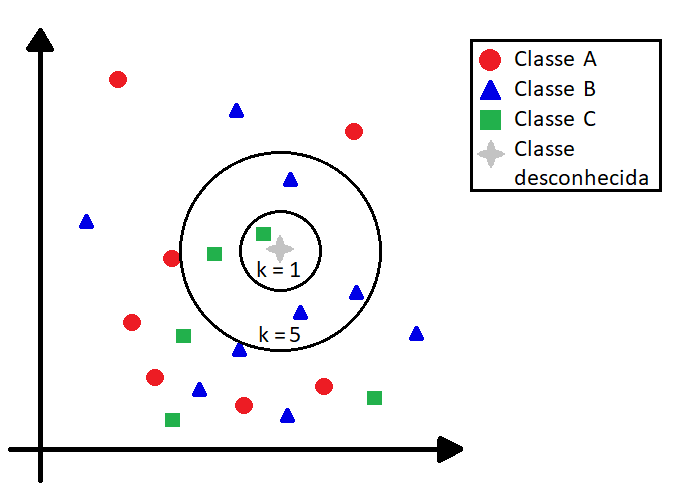
\includegraphics[scale=0.5]{img/knnExample.png}
{\fontsize{11pt}{\baselineskip}\selectfont
\\Fonte: Elaborado pelo autor
}
\end{figure}

\section{Processamento de linguagem natural}
O processamento de linguagem natural (PLN) têm como objetivo tratar os mais diversos aspectos presentes dentro da comunicação humana, tais como sons, palavras, sentenças e discursos, levando em consideração os seus formatos, referências, estruturas, significados, contextos e aplicações. Embora exista outros animais que possuem um vocabulário com centenas de sinais, tais como os elefantes e os golfinhos, somente os seres humanos possuem a capacidade de se comunicar, de forma confiável, em um número ilimitado de mensagens qualitativamente diferentes, sobre um tema qualquer \citep{russell1994inteligencia, gonzalez2003recuperaccao}.

Hoje em dia, com o constante crescimento da rede mundial de computadores, possibilitou o acesso a enumeras páginas de informações na \textit{Web}, no qual quase todas elas estão em um formato de linguagem natural. Entretanto, disponibilidade não significa fácil acesso à informação. Para uma máquina adquirir tal conhecimento, ela precisa ser treinada, de forma exaustiva, para compreender as complexas, e muitas vezes ambíguas, linguagens em que os seres humanos se comunicam.

Segundo \cite{russell1994inteligencia}, as linguagens naturais, tais como o português e o espanhol, não podem ser caracterizadas como um conjunto de sentenças definitivas, pois de acordo com o contexto em que for definida uma sentença de alguma dessas linguagens, ela pode possuir inúmeras interpretações diferentes. Portanto, convém definir um modelo de linguagem natural como uma distribuição de probabilidade sobre sentenças. Existe um famoso ditado popular brasileiro que diz "para um bom entendedor, meia palavra basta", o que pode ser comumente aplicado para nós humanos, que possuímos uma espécie de dispositivo de especialização para aquisição de linguagens \citep{chomsky2014aspects}. Já que meia palavra basta, pode-se concluir que uma sentença de uma linguagem natural não é sempre aleatória, e que sim possui algum grau de previsibilidade e correlação entre a escolha das palavras. Portanto, nos leva a acreditar que palavras similares estejam presentes no mesmo contexto.

O PLN consiste no emprego de um conjunto de técnicas computacionais para aprender, entender e reproduzir uma linguagem natural. No processo de tradução do significado, tratamento de ambiguidade e entre outros desafios, o PLN pode utilizar de conhecimentos linguísticos e métodos estatísticos para resolvê-los. Por exemplo, considere uma análise sobre dois textos semelhantes A e B, no qual desconfia-se que exista possibilidade de plágio. Com o uso de um pré-processamento, seria possível filtrar os textos para remover \textit{Stopwords}, que são palavras funcionais, tais como artigos, preposições e conetivos, que quando analisadas individualmente não possuem grande relevância para o contexto. Após o pré-processamento, é possível aplicar um método da distância mínima de edição, que como o próprio nome diz, significa quantas operações de inserções, remoções ou substituições de caracteres são necessárias para que o texto A torne-se o texto B, ou vice-versa. Uma das tarefas possíveis no PLN é a classificação de texto. Para compreender melhor o processo de aplicação de conhecimentos linguísticos para essa tarefa, é apresentado a seguir uma seção sobre classificação de
texto.

\subsection{Classificação de texto}
Segundo \cite{aggarwal2014data} um dos principais desafios encontrados durante o processo de classificação de texto é sobre o tamanho dos dados tratados, que podem variar de algumas poucas dezenas para milhões de palavras. Esses dados se encontram, quase sempre, de maneira esparsa, ou seja, possuindo baixa frequência de uso. Por outro lado, têm-se muitas vezes uma alta frequência de dados não úteis para tratamento, como as \textit{Stopwords}. Por esse motivo, uma etapa de extração e seleção de características é essencial, e pode gerar benefícios como redução da dimensão do problema, que por sua vez aumenta a velocidade de execução do algoritmo; redução na quantidade total de características; aumento na precisão de predição e acerto; e facilitar a visualização dos dados.

Uma vez escolhido um conjunto de características, é possível aplicar algumas técnicas de classificação de texto, inclusive duas das que já foram abordadas aqui, as redes neurais artificiais e o k-vizinhos mais próximos, nos quais apresentam uma precisão superior a 98\% quando aplicados ao problema de identificação de \textit{e-mail spam} \citep{russell1994inteligencia}.

A classificação ou categorização de texto é a tarefa de, dado algum tipo de texto, decidir a qual conjunto predefinido de classes o mesmo pertence. Por exemplo, decidir a qual linguagem pertence uma sentença ou identificar se um texto de uma chamada de emergência é falsa ou não, são exemplos de classificação de texto.